% !TEX program = xelatex
\documentclass[11pt, a4paper]{article}

\usepackage{fontspec}
\usepackage{xetexko}
\usepackage[margin=2cm, top=2.5cm, bottom=2.5cm]{geometry}
\usepackage{graphicx}
\usepackage{booktabs}
\usepackage{tabularx}
\usepackage{xcolor}
\usepackage{hyperref}
\usepackage{titlesec}
\usepackage{fancyhdr}
\usepackage{enumitem}
\usepackage{float}
\usepackage{caption}
\usepackage{array}
\usepackage{colortbl}
\usepackage{tikz}
\usepackage{multicol}

\setmainfont{Apple SD Gothic Neo}
\setsansfont{Apple SD Gothic Neo}
\setmonofont{Menlo}

\definecolor{darkblue}{HTML}{1A5276}
\definecolor{medblue}{HTML}{2980B9}
\definecolor{lightblue}{HTML}{D4E6F1}
\definecolor{darkgray}{HTML}{2C3E50}
\definecolor{green}{HTML}{27AE60}
\definecolor{orange}{HTML}{E67E22}
\definecolor{red}{HTML}{E74C3C}
\definecolor{purple}{HTML}{8E44AD}
\definecolor{lightgray}{HTML}{F2F3F4}

\hypersetup{colorlinks=true, linkcolor=darkblue, urlcolor=medblue}

\titleformat{\section}
  {\Large\bfseries\color{darkblue}}{\thesection.}{0.5em}{}
  [\vspace{-0.5em}\textcolor{medblue}{\rule{\textwidth}{0.5pt}}]
\titleformat{\subsection}
  {\large\bfseries\color{darkblue}}{\thesubsection}{0.5em}{}

\pagestyle{fancy}
\fancyhf{}
\fancyhead[L]{\small\color{darkgray}AI 기반 인구 변화 예측}
\fancyhead[R]{\small\color{darkgray}한양대 빅데이터마케팅 랩}
\fancyfoot[C]{\small\color{darkgray}\thepage}
\renewcommand{\headrulewidth}{0.4pt}

\newcolumntype{L}[1]{>{\raggedright\arraybackslash}p{#1}}
\newcolumntype{C}[1]{>{\centering\arraybackslash}p{#1}}

\setlength{\parskip}{4pt}

\begin{document}

% ── COVER ──
\thispagestyle{empty}
\begin{center}
\vspace*{2.5cm}

{\fontsize{30}{36}\selectfont\bfseries\color{darkblue}
이 동네, 5년 후에도\\[10pt]
사람이 있을까?}

\vspace{0.8cm}

{\Large\color{darkgray}
전국 3,518개 행정동 · 20년 인구·산업·주거 데이터 · AI 인구 변화 예측}

\vspace{0.6cm}
\textcolor{medblue}{\rule{10cm}{0.8pt}}
\vspace{1.5cm}

\begin{tikzpicture}
\node[fill=lightblue, rounded corners=8pt, minimum width=15.5cm, minimum height=4cm] {
  \begin{minipage}{14.5cm}
  \centering
  \vspace{6pt}
  {\large\bfseries\color{darkblue} 한 눈에 보는 프로젝트}\\[10pt]
  \begin{minipage}[t]{0.24\textwidth}\centering
    {\fontsize{28}{32}\selectfont\bfseries\color{darkblue}3,518}\\[2pt]
    {\small\color{darkgray}행정동 전수 분석}
  \end{minipage}\hfill
  \begin{minipage}[t]{0.24\textwidth}\centering
    {\fontsize{28}{32}\selectfont\bfseries\color{green}20년}\\[2pt]
    {\small\color{darkgray}데이터 (2000$\sim$2021)}
  \end{minipage}\hfill
  \begin{minipage}[t]{0.24\textwidth}\centering
    {\fontsize{28}{32}\selectfont\bfseries\color{darkblue}461개}\\[2pt]
    {\small\color{darkgray}분석 변수}
  \end{minipage}\hfill
  \begin{minipage}[t]{0.24\textwidth}\centering
    {\fontsize{28}{32}\selectfont\bfseries\color{purple}4가지}\\[2pt]
    {\small\color{darkgray}인구 세그먼트 예측}
  \end{minipage}
  \vspace{6pt}
  \end{minipage}
};
\end{tikzpicture}

\vspace{1.5cm}

\begin{minipage}{0.85\textwidth}
\colorbox{lightgray}{%
\begin{minipage}{\textwidth}\vspace{8pt}
\centering
\begin{minipage}{0.9\textwidth}
{\color{darkgray}
매장을 열었는데 몇 년 만에 동네 인구가 줄어서 망했다.\\
10년 장기 임대 계약을 했는데 5년 만에 상권이 죽었다.\\[4pt]
\textbf{지금 사람이 많다고 해서, 5년 후에도 많을 거라는 보장은 없습니다.}\\
AI 모델은 어떤 동네가 성장하고, 어떤 동네가 쇠퇴하는지를 미리 알려줍니다.}
\end{minipage}
\vspace{8pt}
\end{minipage}%
}
\end{minipage}

\vspace{1.5cm}

{\large\color{darkgray}
한양대학교 경영대학 · 빅데이터마케팅 랩 · 임보람 교수\\[4pt]
brlim@hanyang.ac.kr · bigdatamarketinglab.com}
\end{center}

\newpage

% ═══════════════════════════════════════════════════════
\section{지역별 인구 추이 — 이미 갈라지고 있다}

한국 전체 인구는 줄어들고 있지만, 모든 동네가 똑같이 줄어드는 건 아닙니다. 어떤 동네는 여전히 사람이 모이고, 어떤 동네는 빠르게 빠지고 있습니다. 아래 그래프는 세 가지 유형의 지역 인구 추이를 보여줍니다.

\begin{figure}[H]
\centering
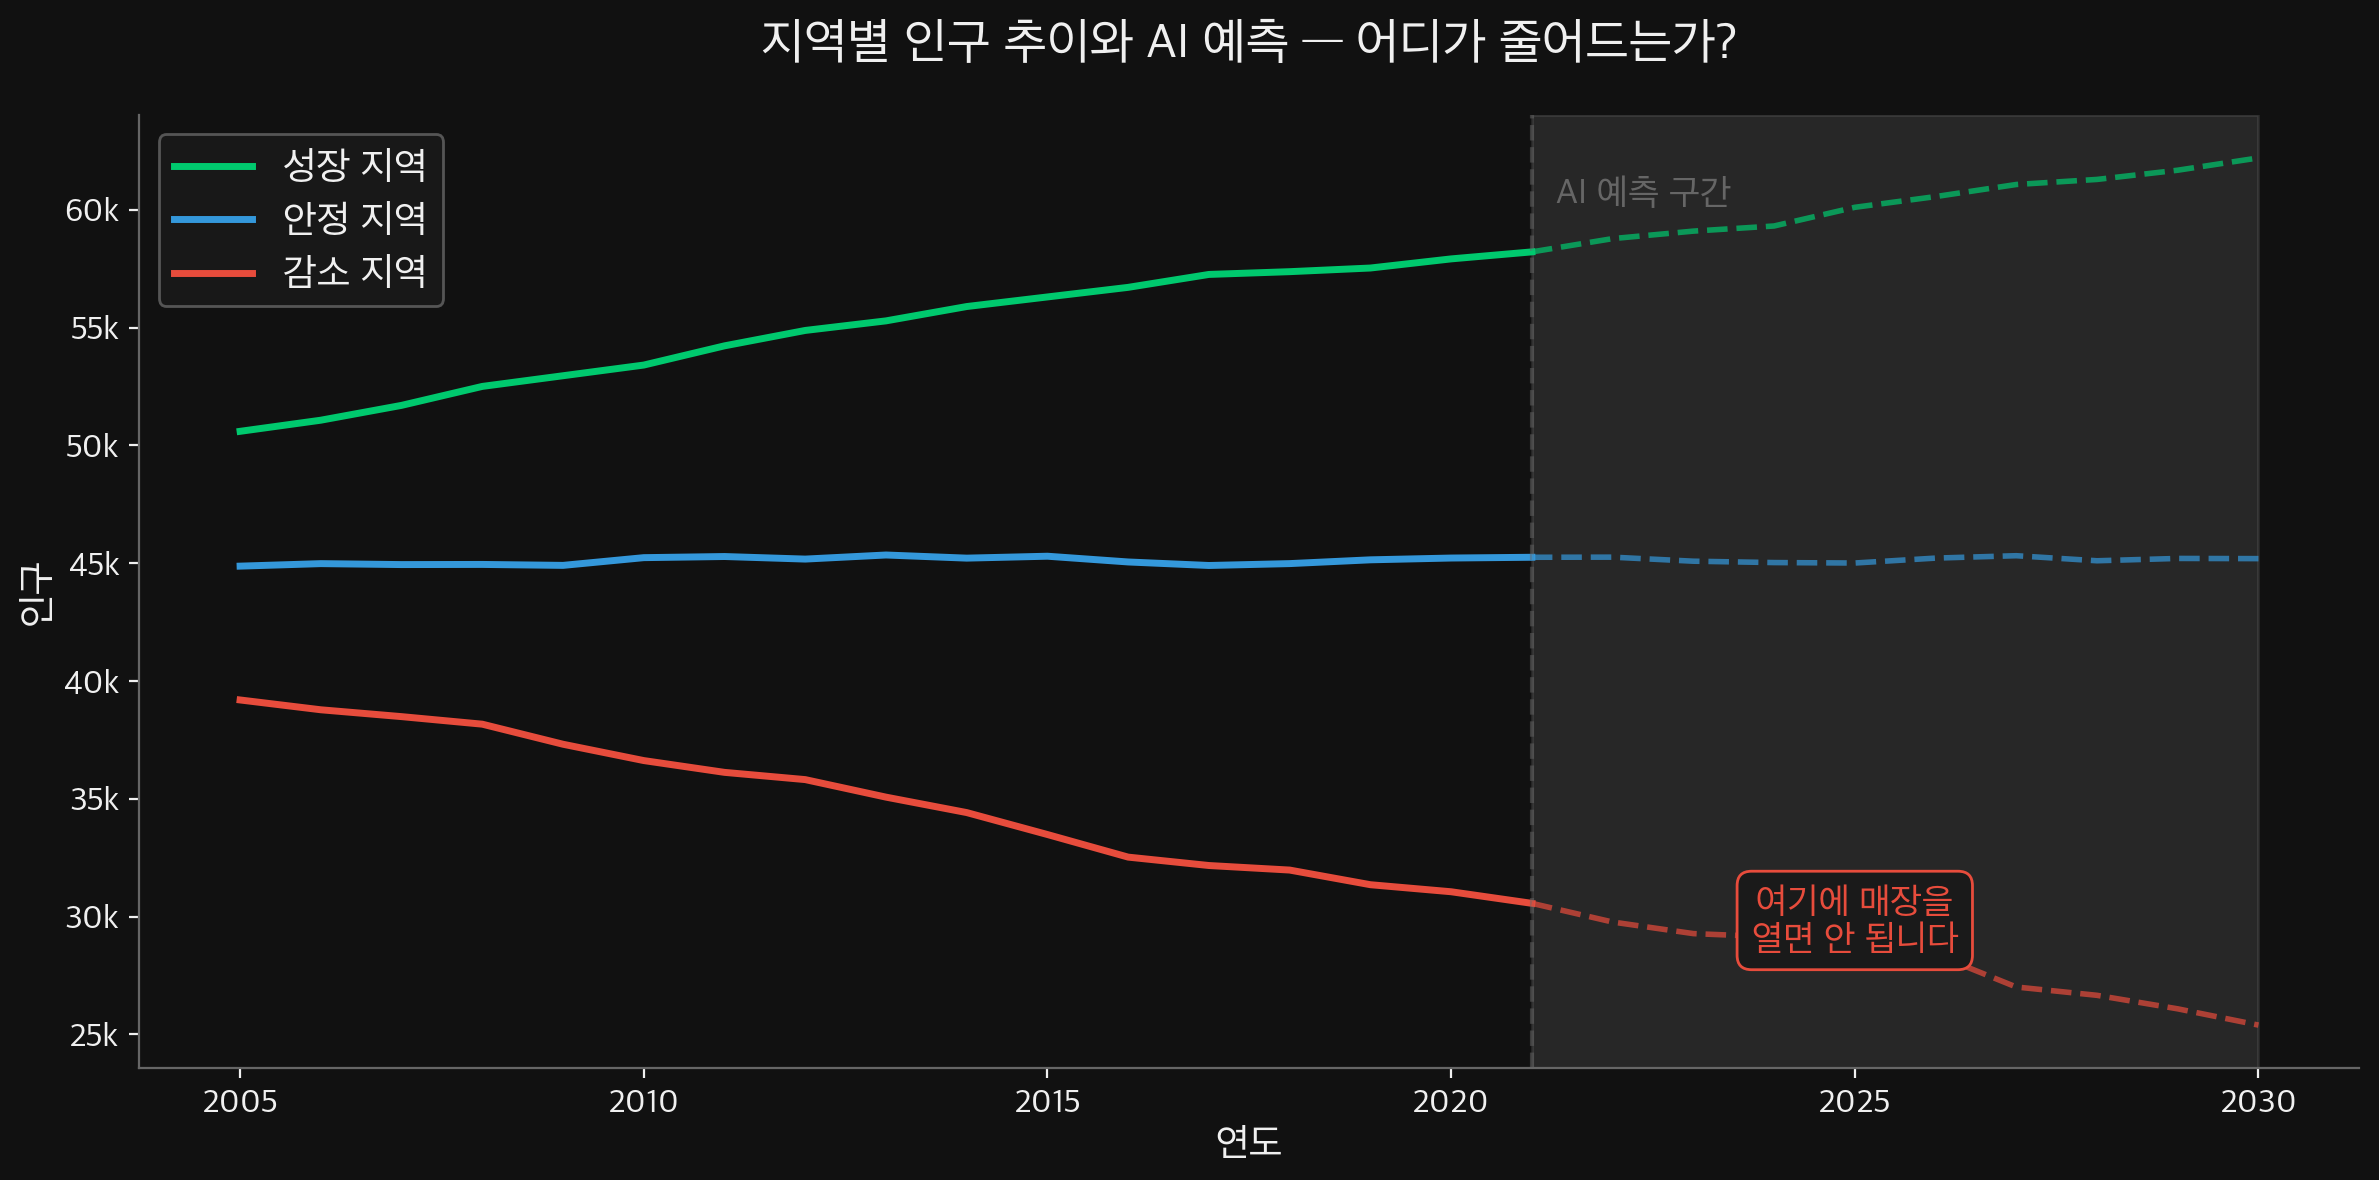
\includegraphics[width=0.88\textwidth]{chart_pop_trajectory.png}
\caption{성장 지역(녹색) vs 안정 지역(파랑) vs 감소 지역(빨강) — 점선은 AI 예측 구간}
\end{figure}

\textbf{핵심:} ``감소 지역''에 매장을 여는 것은 시작부터 불리한 게임입니다.  5년 후 인구가 줄어들 곳에 10년 임대 계약을 하면, 후반 5년은 적자를 각오해야 합니다.

\vspace{0.3cm}

문제는 \textbf{지금 시점에서 어떤 동네가 ``감소 지역''인지 눈으로 보기 어렵다}는 것입니다. 올해 유동인구가 많아도, 그게 5년 후에도 유지된다는 보장이 없습니다. 여기에 AI 예측이 필요합니다.

\subsection{이 프로젝트의 분석 범위}

\begin{table}[H]
\centering
\renewcommand{\arraystretch}{1.2}
\begin{tabularx}{\textwidth}{L{4cm} X}
\toprule
\rowcolor{lightblue} \textbf{항목} & \textbf{내용} \\
\midrule
분석 단위 & 전국 3,518개 읍면동 (행정동) \\
데이터 기간 & 2000$\sim$2021년 (20년간, 5년 단위 + 1년 단위) \\
데이터 출처 & 통계청 인구총조사, 사업체조사, 주택총조사, 가구총조사 \\
변수 수 & 461개 (인구 구조, 가구 형태, 주거 유형, 19개 산업별 사업체/고용 수) \\
예측 모델 & XGBoost (Gradient Boosting Machine) \\
해석 방법 & SHAP (Shapley Additive Explanations) 기반 변수 기여도 분석 \\
검증 방식 & 2005/2010/2015년 데이터로 학습 → \textbf{2020년 실제 변화와 비교} (in-sample validation) \\
\bottomrule
\end{tabularx}
\end{table}

\newpage

% ═══════════════════════════════════════════════════════
\section{무엇을 예측하는가 — 4가지 인구 세그먼트}

전체 인구를 하나로 보면 중요한 신호를 놓칩니다. 전체 인구가 줄지 않더라도 청년이 빠져나가고 있을 수 있고, 고령자 비율이 빠르게 올라가고 있을 수 있습니다. 이 프로젝트는 \textbf{4가지 인구 세그먼트를 각각 별도로 예측}합니다.

\begin{table}[H]
\centering
\renewcommand{\arraystretch}{1.5}
\large
\begin{tabular}{L{4cm} C{2.5cm} C{2.5cm} L{5cm}}
\toprule
\rowcolor{lightblue} \textbf{세그먼트} & \textbf{예측 정확도} & \textbf{RMSE} & \textbf{이것을 알면} \\
\midrule
\textbf{고령 인구} & \textcolor{purple}{\textbf{R² 50.0\%}} & 20.86 & 고령화가 얼마나 빠르게 진행되는가 \\[4pt]
\textbf{청년 (20$\sim$34세)} & \textcolor{darkblue}{\textbf{R² 47.8\%}} & 36.58 & 젊은 인구가 떠나고 있는가, 들어오고 있는가 \\[4pt]
\textbf{전체 인구 유입} & \textcolor{green}{\textbf{R² 47.3\%}} & 24.46 & 동네 전체로 사람이 모이는가, 빠지는가 \\[4pt]
\textbf{영유아 (0$\sim$4세)} & \textcolor{orange}{\textbf{R² 36.4\%}} & 47.22 & 이 동네에 아이를 키우는 가구가 있는가 \\
\bottomrule
\end{tabular}
\caption{5년 후 인구 변화 예측 정확도 — 2020년 실제 데이터 대비 검증}
\end{table}

\begin{figure}[H]
\centering
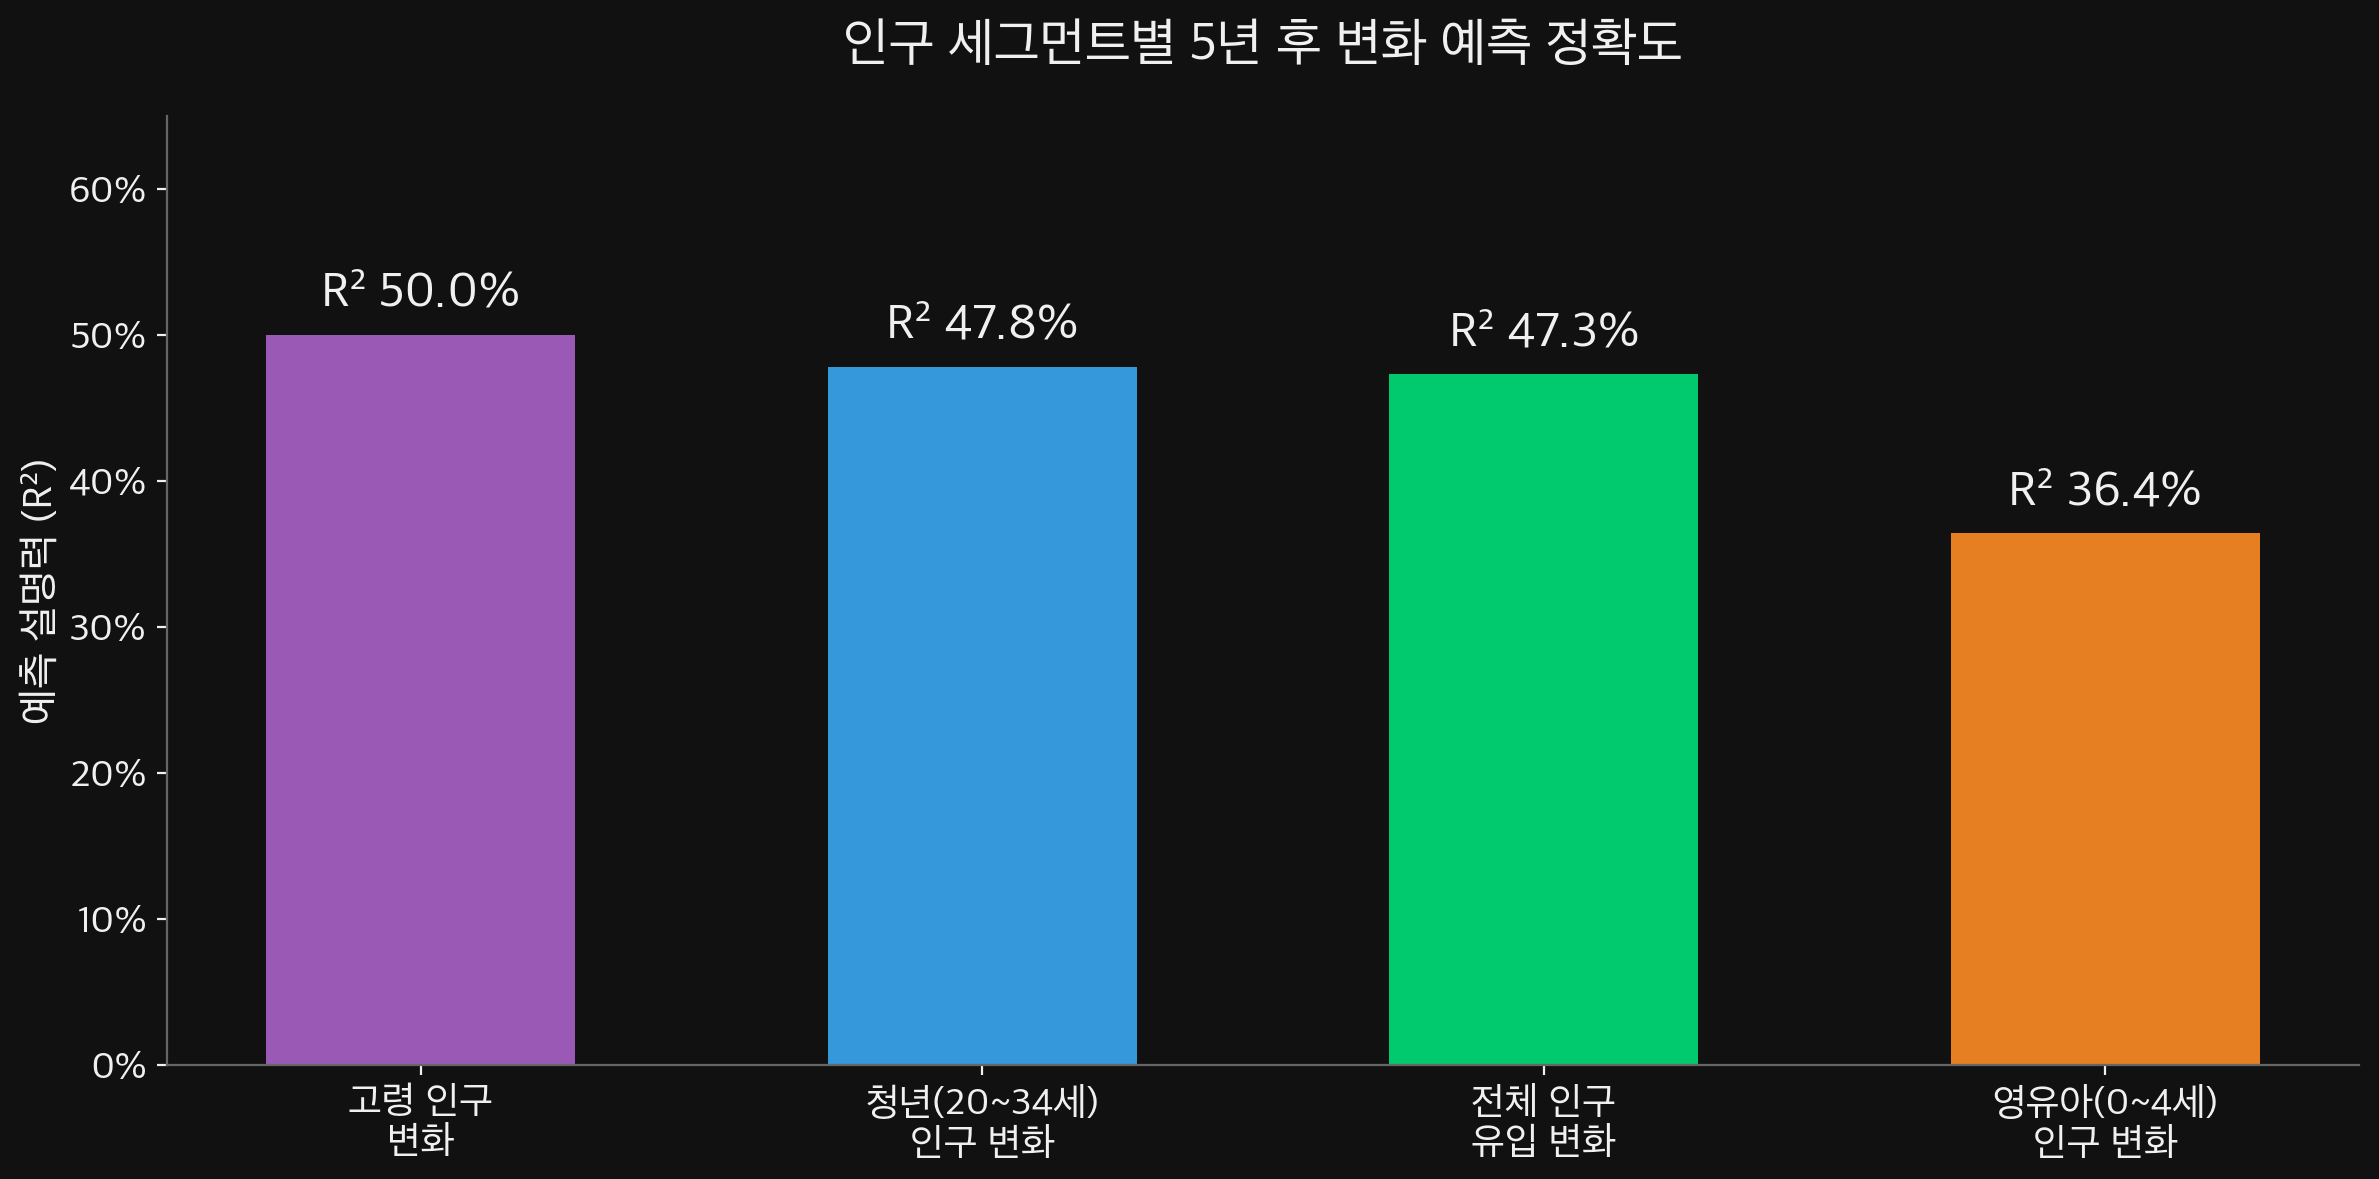
\includegraphics[width=0.88\textwidth]{chart_segment_accuracy.png}
\caption{인구 세그먼트별 5년 후 예측 정확도 (R²)}
\end{figure}

\subsection{왜 세그먼트별로 따로 보는가}

\begin{itemize}[itemsep=4pt, leftmargin=2em]
  \item \textbf{프랜차이즈 매장:} 주 소비층이 20$\sim$34세라면, 전체 인구가 아니라 \textbf{청년 인구 추이}가 중요
  \item \textbf{키즈카페·학원:} 영유아·학령인구가 핵심 → 영유아 세그먼트
  \item \textbf{실버 서비스:} 고령 인구가 늘어나는 곳이 시장 → 고령 세그먼트
  \item \textbf{부동산 투자:} 전체 인구 유입이 있는 곳이 가치 상승 → 전체 세그먼트
\end{itemize}

\textbf{같은 동네라도 세그먼트에 따라 진단이 다릅니다.} 전체 인구는 안정적인데 청년만 빠져나가는 동네, 전체 인구는 줄고 있는데 고령자는 오히려 느는 동네 — 이런 차이를 잡아내는 것이 세그먼트별 예측의 핵심입니다.

\newpage

% ═══════════════════════════════════════════════════════
\section{어떤 동네가 살아남는가 — 핵심 요인 분석}

461개 변수를 동시에 분석했습니다. AI 모델이 인구 변화를 예측할 때 어떤 정보를 가장 많이 참고하는지를 SHAP 기법으로 분해한 결과입니다.

\begin{figure}[H]
\centering
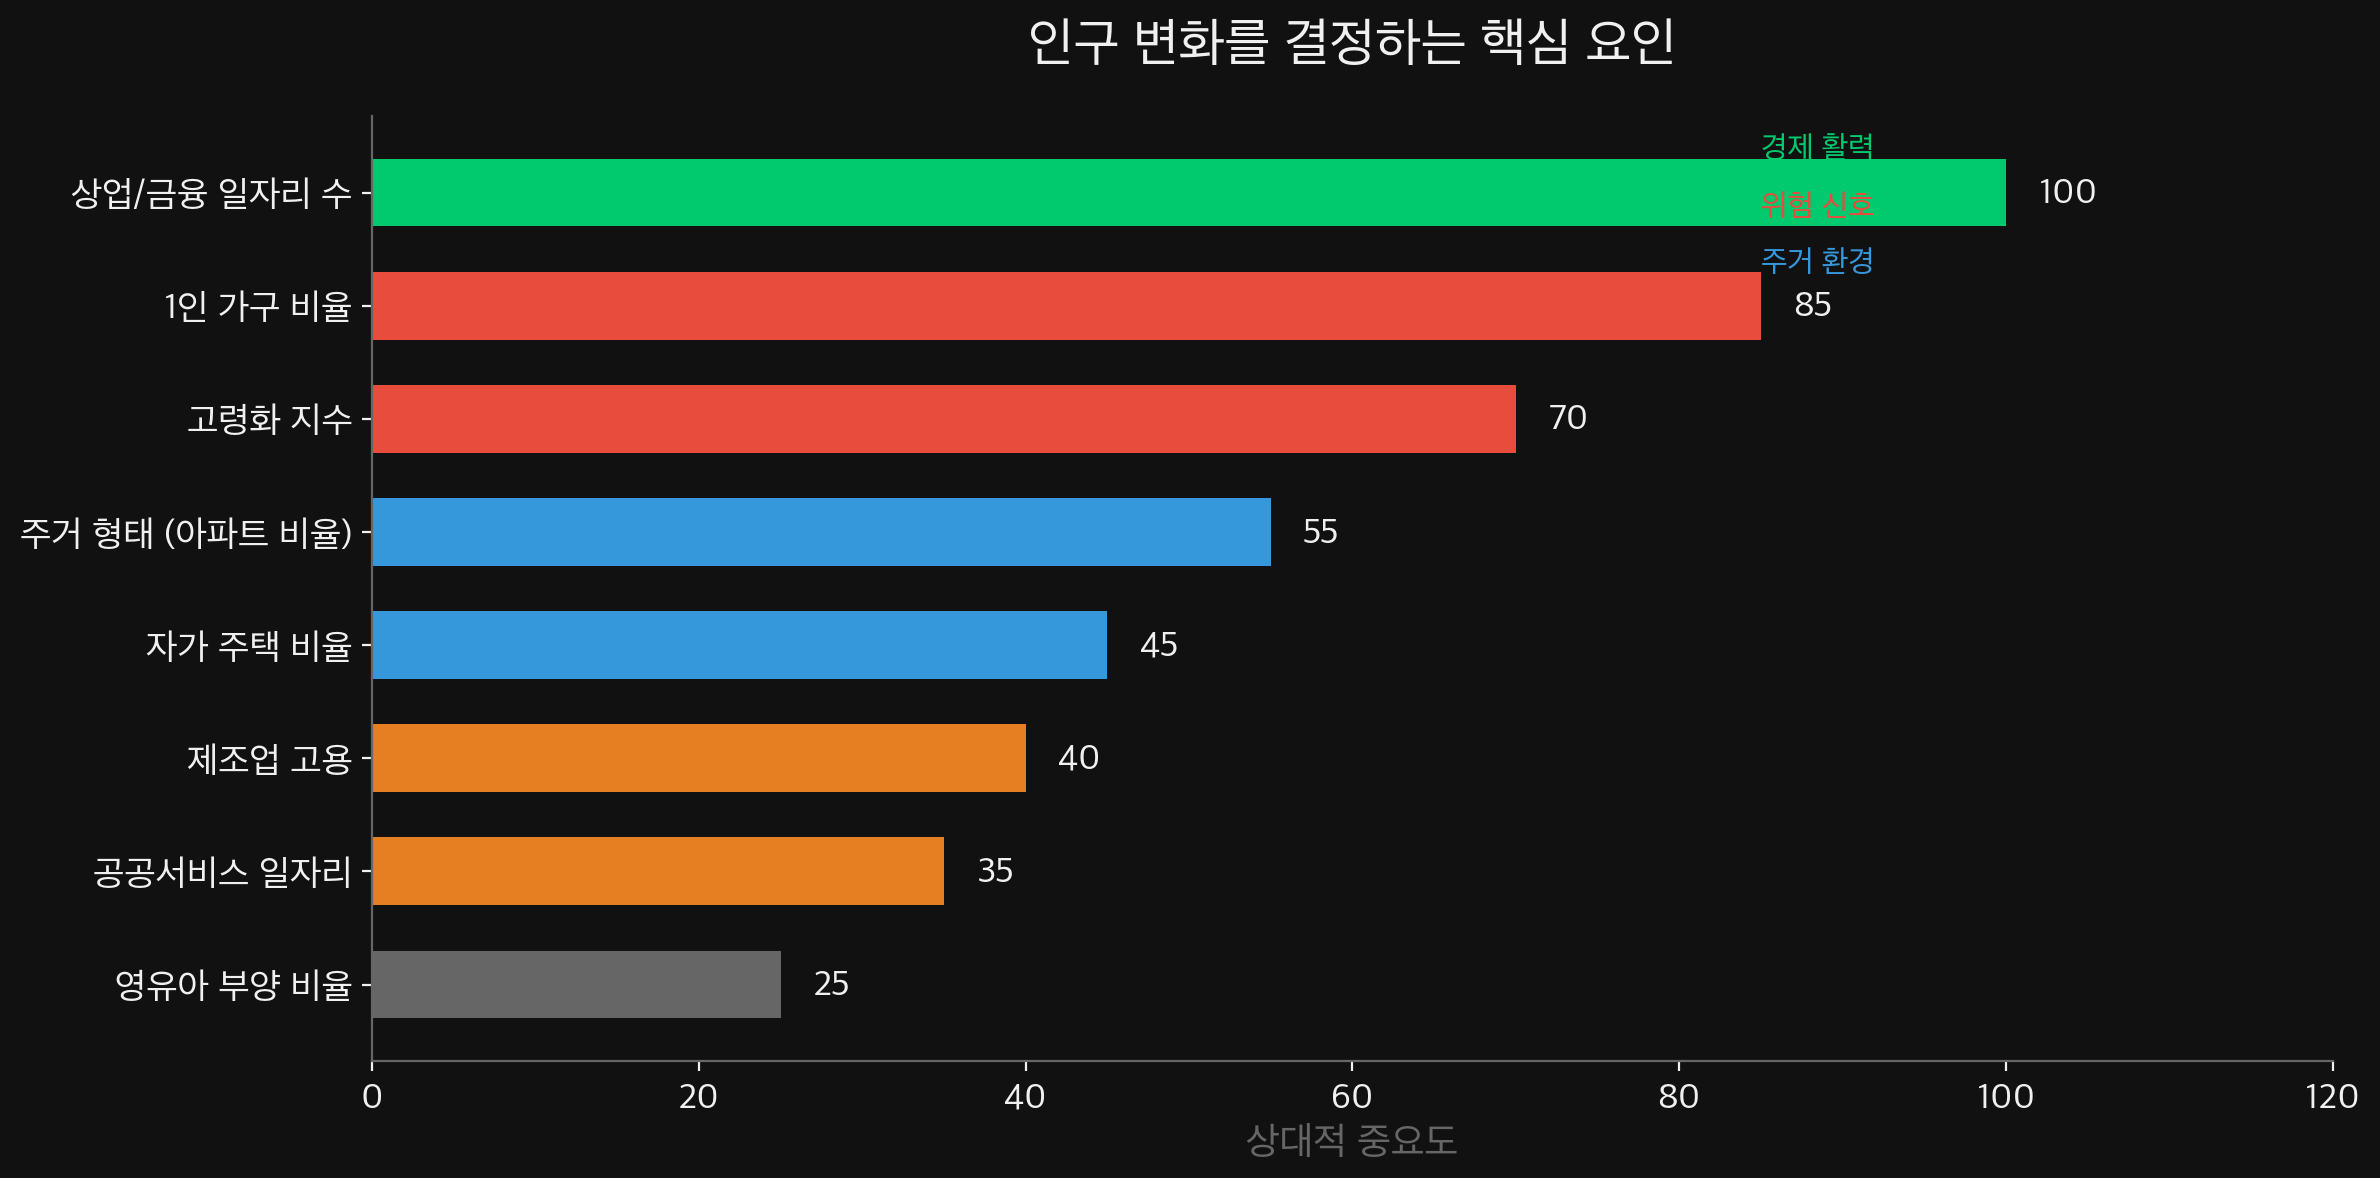
\includegraphics[width=0.88\textwidth]{chart_pop_factors.png}
\caption{인구 변화를 결정하는 핵심 요인 (SHAP 기반 중요도)}
\end{figure}

\subsection{경제 활력 — 일자리가 있는 동네에 사람이 모인다}

\begin{table}[H]
\centering
\renewcommand{\arraystretch}{1.3}
\begin{tabularx}{\textwidth}{L{4.5cm} C{2.5cm} X}
\toprule
\rowcolor{lightblue} \textbf{요인} & \textbf{기여도} & \textbf{해석} \\
\midrule
\textbf{상업·소매 사업체 수} & \textcolor{green}{\textbf{1위}} & 상점, 식당, 소매점이 많은 동네 = 경제 활동이 활발 = 사람이 모임 \\[4pt]
\textbf{금융·전문서비스 고용} & 높음 & 사무직 일자리가 있는 동네는 청년 유입이 강함 \\[4pt]
\textbf{제조업 고용 변화} & 중간 & 제조업 일자리가 줄면, 해당 지역 인구도 줄어드는 강한 상관 \\[4pt]
\textbf{공공서비스 일자리} & 중간 & 병원, 학교, 관공서가 있는 곳은 인구가 상대적으로 안정 \\
\bottomrule
\end{tabularx}
\end{table}

\subsection{위험 신호 — 이런 동네는 인구가 줄어든다}

\begin{table}[H]
\centering
\renewcommand{\arraystretch}{1.3}
\begin{tabularx}{\textwidth}{L{4.5cm} C{2.5cm} X}
\toprule
\rowcolor{lightblue} \textbf{요인} & \textbf{방향} & \textbf{해석} \\
\midrule
\textbf{1인 가구 비율} & \textcolor{red}{\textbf{높으면 위험}} & 1인 가구는 이동이 쉬움 → 조건이 나빠지면 바로 떠남 \\[4pt]
\textbf{고령화 지수 (노인 비율)} & \textcolor{red}{\textbf{높으면 위험}} & 노인 비율 ↑ → 상권 위축 → 청년 이탈 → 악순환 \\[4pt]
\textbf{영유아 부양 비율} & 낮으면 위험 & 아이가 없는 동네 = 젊은 가구가 없다는 신호 \\
\bottomrule
\end{tabularx}
\end{table}

\subsection{주거 환경 — 구조가 인구를 결정한다}

\begin{table}[H]
\centering
\renewcommand{\arraystretch}{1.3}
\begin{tabularx}{\textwidth}{L{4.5cm} C{2.5cm} X}
\toprule
\rowcolor{lightblue} \textbf{요인} & \textbf{방향} & \textbf{해석} \\
\midrule
\textbf{아파트 비율} & 높으면 안정 & 아파트 단지 = 가족 단위 거주 → 인구 안정적 \\[4pt]
\textbf{자가 주택 비율} & 높으면 안정 & 자가 소유자는 쉽게 떠나지 않음 → 인구 유지 \\[4pt]
\textbf{단독주택 비율} & 높으면 주의 & 노후 주거지 = 재개발 or 인구 감소 \\
\bottomrule
\end{tabularx}
\end{table}

\colorbox{lightblue}{%
\begin{minipage}{0.95\textwidth}\vspace{8pt}
\textbf{핵심:} 단순히 ``줄어든다/안 줄어든다''가 아니라 \textbf{왜 줄어드는지}를 압니다. 일자리가 문제인지, 주거 구조가 문제인지, 고령화가 문제인지 — 원인에 따라 대응이 달라집니다.
\vspace{8pt}
\end{minipage}%
}

\newpage

% ═══════════════════════════════════════════════════════
\section{프랜차이즈·리테일에 이렇게 씁니다}

\begin{figure}[H]
\centering
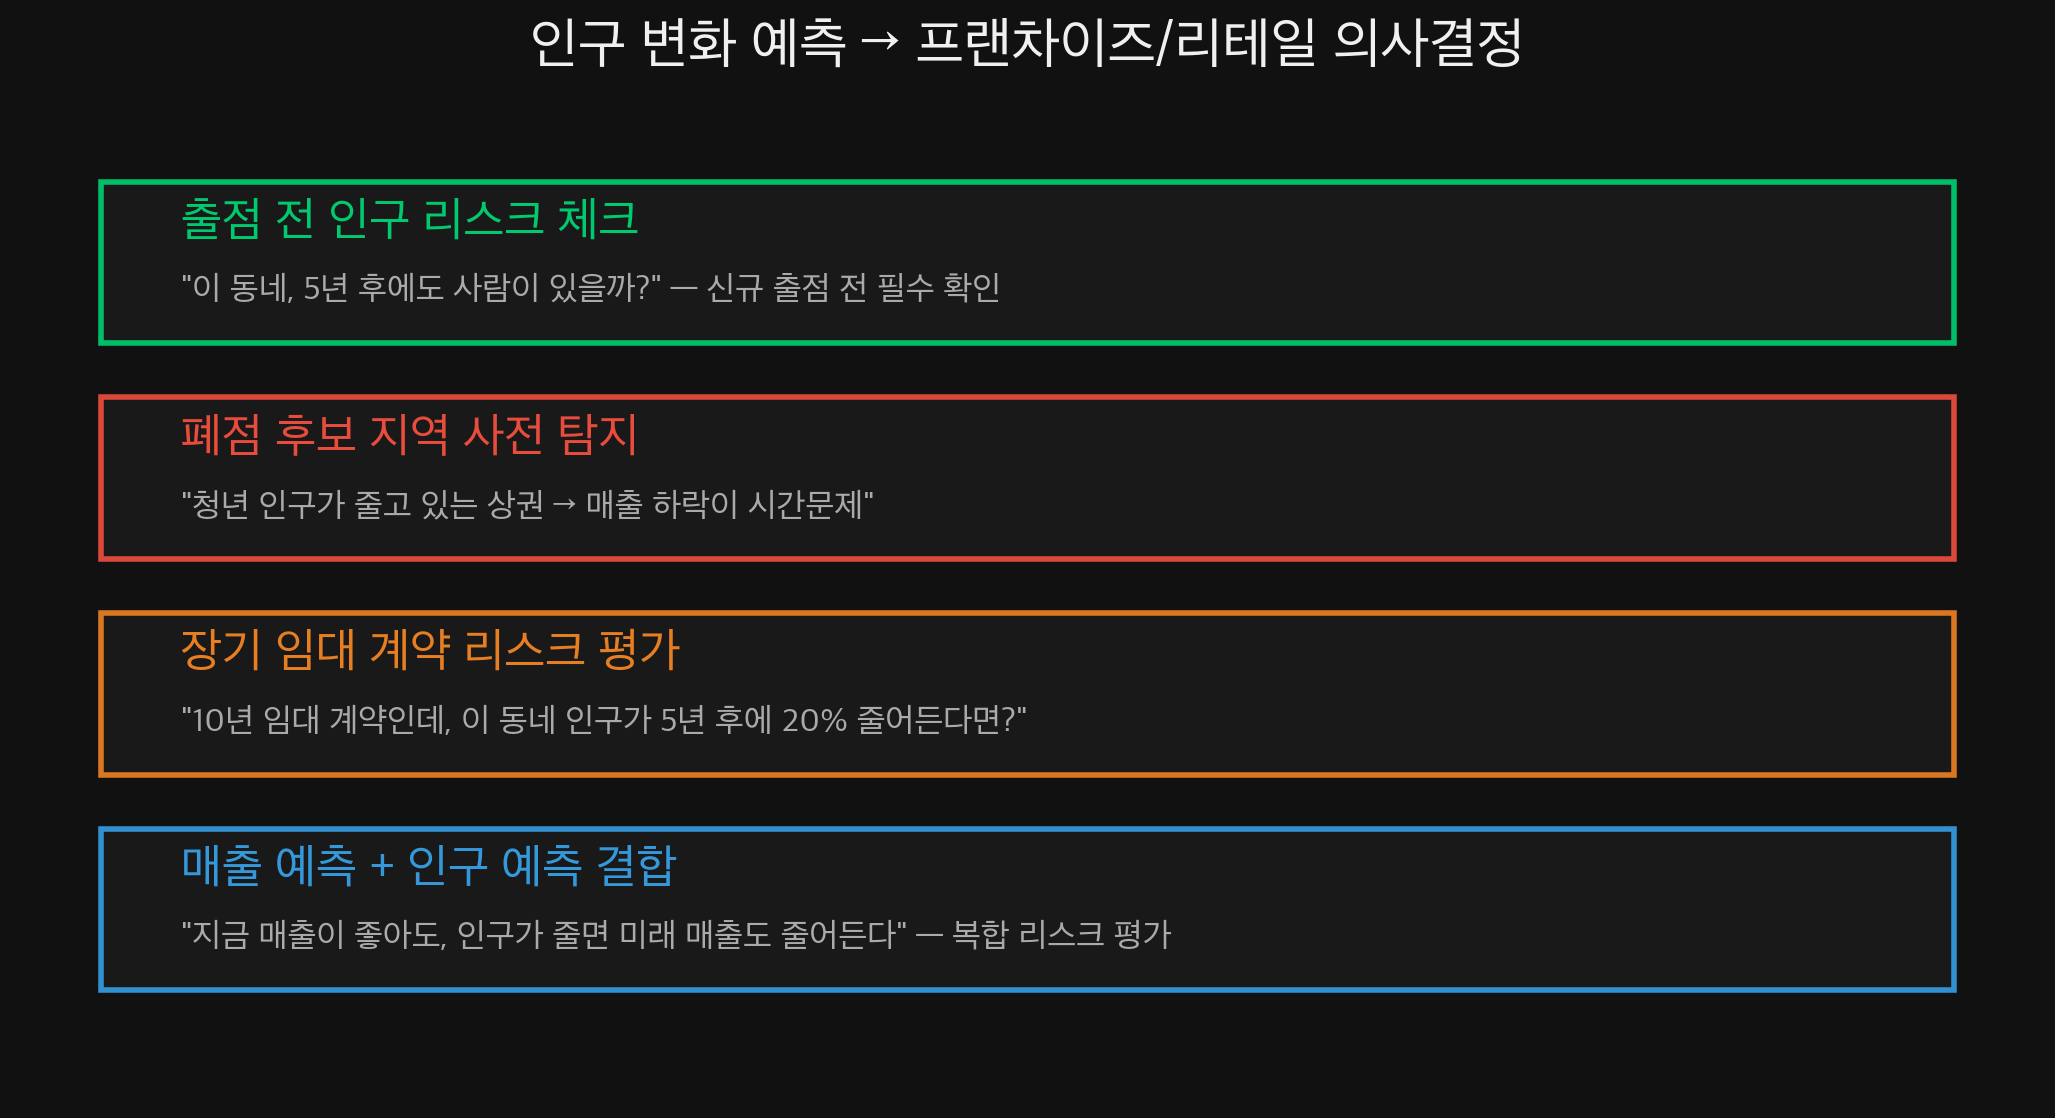
\includegraphics[width=0.9\textwidth]{chart_pop_applications.png}
\caption{인구 예측의 비즈니스 활용}
\end{figure}

\subsection{출점 전 인구 리스크 체크}

신규 매장 출점을 검토할 때, 현재 상권 분석만으로는 부족합니다. ``지금 사람이 많은가''가 아니라 \textbf{``5년 후에도 사람이 있을 것인가''}를 확인해야 합니다.

\begin{itemize}[itemsep=3pt, leftmargin=2em]
  \item 출점 후보지의 행정동 코드를 입력하면 → 5년 후 인구 변화율 예측
  \item 청년 인구, 고령 인구, 영유아 인구 각각의 추이를 확인
  \item 주변 경쟁 후보지 대비 인구 리스크 비교 가능
\end{itemize}

\subsection{폐점 후보 지역 사전 탐지}

이미 운영 중인 매장 중에서, 위치한 동네의 인구가 줄어들고 있는 곳을 사전에 파악합니다. 매출이 아직 떨어지지 않았더라도, \textbf{인구가 줄면 매출 하락은 시간문제}입니다.

\begin{itemize}[itemsep=3pt, leftmargin=2em]
  \item 전체 매장 리스트의 행정동을 일괄 분석
  \item ``이 매장이 위치한 동네의 청년 인구가 5년간 15\% 줄 것으로 예측'' → 주의 리스트에 등록
  \item 매출 데이터와 결합하면, 인구 감소 + 매출 하락의 복합 경고가 가능
\end{itemize}

\subsection{장기 임대 계약 리스크 평가}

5년 이상 장기 임대 계약을 체결할 때, 해당 동네의 인구 전망은 계약 조건만큼 중요합니다. 임대료는 고정인데 인구가 줄면, 매출로 임대료를 감당하지 못하는 상황이 발생합니다.

\subsection{매출 예측과의 결합 — 완전한 의사결정}

\colorbox{lightblue}{%
\begin{minipage}{0.95\textwidth}\vspace{8pt}
\centering
{\large\bfseries\color{darkblue} 매출 예측 + 인구 예측 = 완전한 출점 의사결정}\\[8pt]
\begin{minipage}{0.9\textwidth}
\begin{itemize}[itemsep=4pt, leftmargin=1.5em]
  \item \textbf{매출 예측만:} ``이 매장은 지금 잘 팔리고 있다'' → 하지만 내년에도?
  \item \textbf{인구 예측만:} ``이 동네 인구가 줄고 있다'' → 하지만 매출에 얼마나 영향?
  \item \textbf{결합:} ``지금 매출이 좋지만, 인구가 줄고 있어서 2년 후 매출이 20\% 감소할 것'' → \textbf{구체적 의사결정 가능}
\end{itemize}
\end{minipage}
\vspace{8pt}
\end{minipage}%
}

BDM Lab은 \textbf{매출 예측 (R² 98\%)}과 \textbf{인구 예측}을 모두 수행할 수 있는 역량을 보유하고 있으며, 두 가지를 결합한 종합 리스크 평가가 가능합니다.

\newpage

% ═══════════════════════════════════════════════════════
\section{분석 방법 상세}

\subsection{데이터}

\begin{table}[H]
\centering
\renewcommand{\arraystretch}{1.2}
\begin{tabularx}{\textwidth}{L{4.5cm} X}
\toprule
\rowcolor{lightblue} \textbf{데이터 카테고리} & \textbf{포함 변수 (예시)} \\
\midrule
인구 구조 & 총인구, 연령별 인구 (5세 단위), 성별 인구, 인구이동 \\[3pt]
가구 형태 & 1인 가구 비율, 가구 수, 가구 유형 (1세대/2세대/3세대) \\[3pt]
주거 환경 & 아파트 비율, 단독주택 비율, 자가/전세/월세, 주택 면적 분포 \\[3pt]
산업 구조 (19개 업종) & 농림어업, 제조업, 건설업, 도소매업, 금융업, 공공서비스 등 사업체 수 \\[3pt]
고용 구조 (19개 업종) & 업종별 종사자 수, 고용 변화율 \\[3pt]
파생 지표 & 고령화 지수, 유소년 부양비, 노년 부양비, 1인 가구 비율 등 \\
\bottomrule
\end{tabularx}
\end{table}

\subsection{모델 구조}

\begin{table}[H]
\centering
\renewcommand{\arraystretch}{1.3}
\begin{tabularx}{\textwidth}{L{4cm} X}
\toprule
\rowcolor{lightblue} \textbf{항목} & \textbf{내용} \\
\midrule
\textbf{기본 모델 (Baseline)} & 1인 가구 비율, 자가 주택 비율, 아파트 비율, 단독주택 비율, 고령 부양비, 유소년 부양비, 1인 남성 비율, 1인 여성 비율 (8개 변수) \\[4pt]
\textbf{확장 모델} & Baseline + 19개 산업별 사업체 수 + 19개 산업별 종사자 수 + 변화율 \\[4pt]
\textbf{최고 성능 조합} & Baseline + 전 산업 종사자 변화율 → R² 47.3\%$\sim$50.0\% \\[4pt]
\textbf{알고리즘} & XGBoost (reg:squarederror, tree\_method=hist) \\[4pt]
\textbf{해석} & SHAP (TreeExplainer) → 변수별 기여도 정량 분해 \\
\bottomrule
\end{tabularx}
\end{table}

\subsection{검증 방식}

\begin{itemize}[itemsep=4pt, leftmargin=2em]
  \item \textbf{학습 데이터:} 2005, 2010, 2015년의 인구·산업·주거 변수
  \item \textbf{검증 데이터:} 2020년의 실제 인구 변화 (학습에 사용하지 않음)
  \item \textbf{예측 대상:} ``2015년 시점의 변수로, 2020년의 인구 변화를 맞출 수 있는가?''
  \item \textbf{메트릭:} R² (결정계수), RMSE (평균 제곱근 오차)
\end{itemize}

즉, \textbf{과거 데이터만으로 미래를 맞출 수 있는지}를 검증한 것이며, 미래 정보는 전혀 사용하지 않았습니다.

\vspace{1cm}

\begin{center}
\textcolor{medblue}{\rule{8cm}{0.8pt}}

\vspace{0.8cm}

{\Large\bfseries\color{darkblue} 문의}

\vspace{0.4cm}

{\large\color{darkgray}
임보람 교수\\[3pt]
한양대학교 경영대학 · 빅데이터마케팅 랩\\[6pt]
brlim@hanyang.ac.kr\\[3pt]
bigdatamarketinglab.com}
\end{center}

\end{document}
